\chapter{Background Research}\label{ch:Background Research}
This chapter provides some background research on the conclusions of the literature review. Mainly looking into the algorithm a how training the model works. All things that were investigated during the implementation stage of the research artefact are discussed in this chapter.

\section{Algorithm}
The algorithm chosen from the papers in the literature review to be most relevant to use was the Neural Network algorithm. This algorithm can be used for both regression and classification tasks. In this instance a classification neural network algorithm is to be used. A neural network is a parallel, distributed information processing structure consisting of processing elements (units or nodes) interconnected together \cite{118638}. Examples of different neural network architectures can be seen in figure \ref{fig:NNA} below. Taken from \cite{485891} 
\begin{figure}[h!]
  \centering
  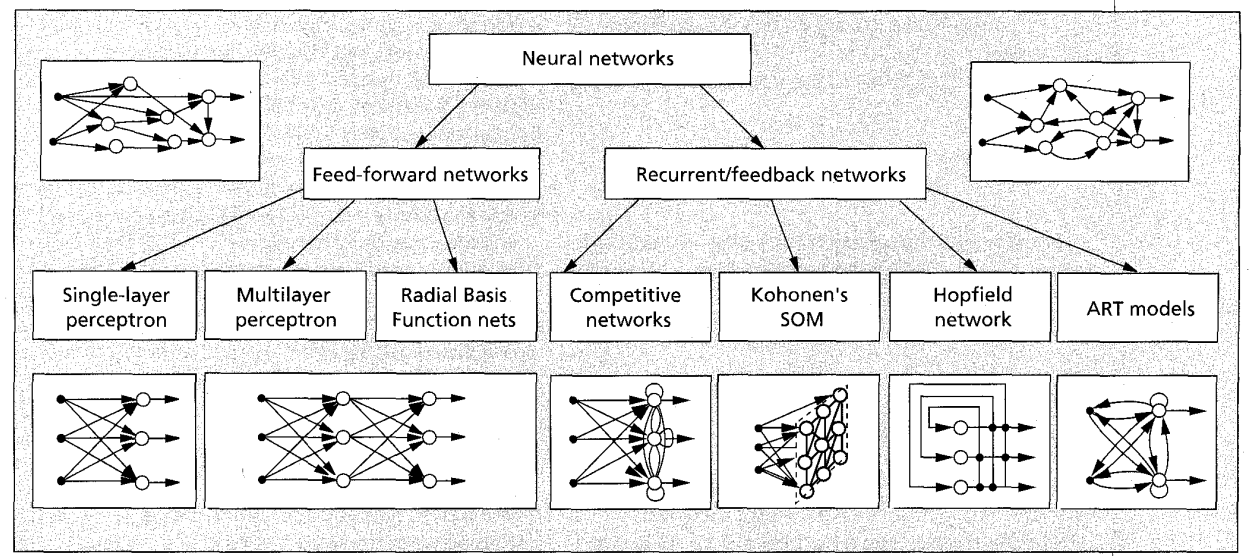
\includegraphics[width = (\textwidth)/2]{nnarc.png}
  \caption{Examples of different neural network architectures}
  \label{fig:NNA}
\end{figure}

A neural network works by passing in the data to the input layer which passes the data onto the hidden layer(s) ( the more complex a Neural Network, the more hidden layers it may have). On the hidden layer the neuron calculates the sum of the weights passed onto it. This then triggers an activation function which,the goal of an activation function is to define the output of a neuron's weighted input \cite{samatin_njikam_zhao_2016}. Once the prediction has been made the output is compared to the target input.The difference between the two patterns of output then determines how the weights are altered. Each particular recipe for change constitutes a learning rule \cite{Gurney1997AnIT}.

\section{Neural Network Learning Process}
The main learning process for a classification Neural Network (NN) involves a type of learning call supervised learning. In supervised leaning the training set includes the input patterns as well as the correct results. then after the output is given if the output is wrong the weights can be adjusted according to the difference \cite{kriesel}. A flowchart of supervised leaning can be seen below in figure \ref{fig:slfc}. Taken from \cite{seb}. 
\begin{figure}[h!]
  \centering
  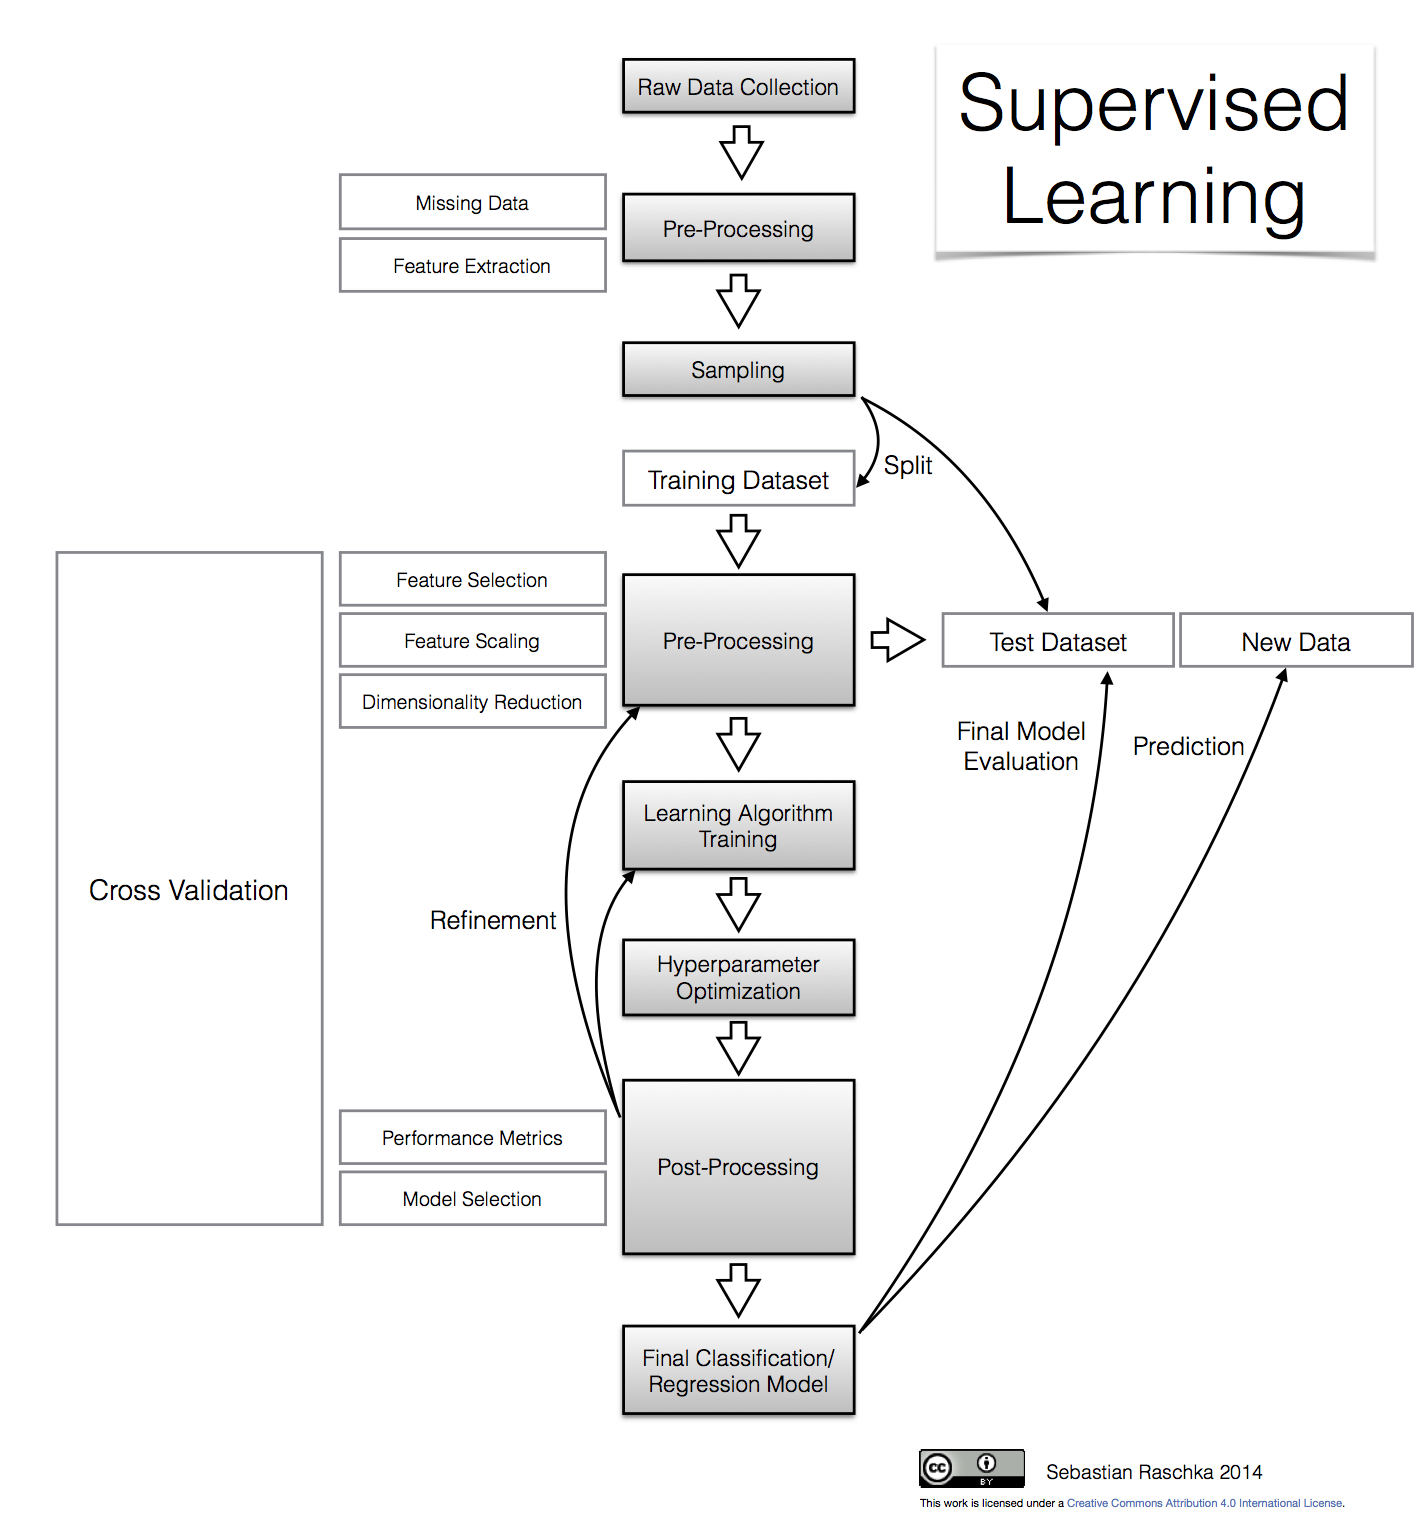
\includegraphics[width = (\textwidth)/2]{supervisedlearningflowchart.png}
  \caption{A flowchart showing the supervised learning process}
  \label{fig:slfc}
\end{figure}

\section{Conclusions}

With this extra background research and the conclusions of the literature review the design stages of the research artefact model can take place. Following on from this the research means that the knowledge needed for the implementation of the research artefact software can take place with ease. 




